\chapter{Modeling}
Im folgenden werden verschiedene Modelle aufgebaut, um auf dem gegeben Datensatz aus dem vorangegangen Kapitel vorherzusagen, wie sich der Aktienpreis ändert. Dabei wird die Aktienpreisänderung fokussiert, und nicht der eigentlichen Aktienpreis. Also (1) steigend, (-1) fallend oder (0) unverändert. Die Zielvariable ist also stehts der im Datensatz vorhandene stockPrice\_Change.
\section{Sentiment Analyse, Lineare Regression}
Zunächst betrachten wir die Änderungen des Aktienpreises anhand des im Kapitel der Data Preparation berechneten Sentiment auf wörterbuchbasis.

\subsection{Model bauen}
Durchschnittlich liegt der Sentiment-Score der Headlines bei -0.056242, der kleinste Sentiment-Score beträgt -4.2500, der größte 3.375.	
Nach kurzer Betrachtung der Binären Zuordnungen stockPrice\_Change und senti\_Binary ist zu erkennen, dass 54086 Sentiments der Headlines von 161478 positiv mit einem Aktienanstieg korrelieren. Das entspricht etwa 33\%. Das bedeutet, bei positiven Sentiment steigt die Aktie, bei negativen Sentiment fällt diese. Hingegen korellieren rund 20\% der Headlines, bzw. deren Sentiment, negativ mit einem Aktienanstieg.\\
Um dieses Vorgehen weiter zu verfeinern, wird ein lineares Regressionsmodell aufgebaut \citep{linearRegression}. Zunächst nehmen wir den Sentiment-Score der Headline als Predictor, als Input-Varible, die Zielvariable bleibt unverändert. Das lineare Regressionsmodell berechnet nun die mögliche Gewichtung der Predictoren um die Zielvariable herzuleiten \citep{cakra_trisedya2016}. Durch die Differenzierung des Sentiment-Score in positiv und negativ, erhalten wir zwei Predictoren zur selben Zielvariable. 
In einem weiteren Modell wird zusätzlich der Aktienpreis zum Zeitpunkt der Börseneröffnung als Predictor herangezogen, so werden also weitere äußere Umstände in das Modell mit einbezogen. Letztlich ergänzen wir dem Datensatz die Anzahl der Veröffentlichungen, also der Headlines, zur selben Aktie an diesem Tag und nutzen diese zusammen mit dem positiven und negativen Sentiment-Score als Predictoren. So können Zusammenhänge zwischen dem Aktienpreis und der wiederholten Erwähnung einer Aktie in das Modell mit einfließen.

\subsection{Model bewerten}
Die reine Korrelation ist wenig Aussagekräftig, da nur 33\% einen direkten Zusammenhang aufweisen. Dies liegt primär an den 61614 Headlines, welche einen Sentiment Score von 0 besitzen und somit nicht zu deuten sind. Dies widerum liegt ist vermutlich auf das nicht auf den Finanzmarkt spezialisierte Sentiment-Dictionary zurück zuführen \citep{ronenFeldman2013}
Um die entstandenen Modelle nun mit einander zu vergleichen und zu bewerten, wenden wir die jeweiligen Modelle, trainiert auf einem zufälligem train\_set von rund 70\% des gesamt Datensatzes, auf einem test\_set (die restlichen 30\% des Datensatzes) an. Somit enthält der test\_set Datensatz vier Predictions und den tatsächlichen StockPrice\_Change.\\
Wie in \ref{evaluationSentiment} zu erkennen steigt die Accuracy von Modell zu Modell, liegt aber immer unter 40\%. Die Accuracy sagt aus, wie viele der Vorhersagen den tatsächlichen Werten entsprechen. Konkret: 
\begin{align}
    accuracy\: { = }\: \frac{Anzahl\:korrekter\:Vorhersagen}{Gesamtanzahl\:Vorhersagen}
    \label{TF Formel}
\end{align}
Eine solch niedrige Accuracy zeigt also, das die verwendeten Predictoren, nicht genau genug sind oder nicht ausreichen, um zuverlässig den tatsächlichen Wert zu berechnen. Dies wird auch durch den RMSE, dem Root Mean Squared Error, und dem $\text{R}^2$ gezeigt. Der hohe RMSE un der niedrige $\text{R}^2$ sagen aus, dass das Modell eben nicht gut an die tatsächlichen werte angepasst ist. An den Koeffizienten ist auch zu sehen, das jeder der Eingabevariablen nur einen geringen Einfluss auf die Zeilvariable hat \citep{uyanik_gueler2013}.
\begin{figure}[b]
    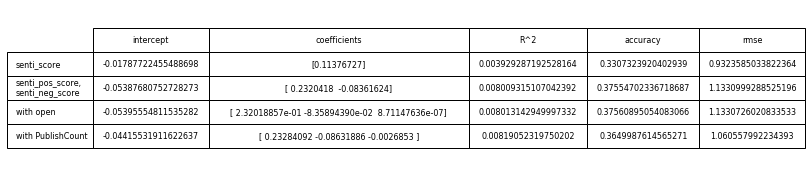
\includegraphics[width=1\textwidth]{img/evaluation_sentiment_Modelling.png}
    \caption{Vergleich von vier Linearen Regressionen}
    \label{evaluationSentiment}
\end{figure}
\\Schlussendlich ist zu erkennen, das der Zusammenhang des Sentiments und der Aktienpreis Entwicklung unter den hier herrschenden Bedingungen nicht eindeutig nachzuweisen ist.

\section{Bag-Of-Words und TF-IDF mit Random Forest Regression}
Neben der wörterbuchbasierten Methode, betrachten wir in unserer zweiten Analyse den Datensatz auf Grundlage des Bag-Of-Words Modells. Hierbei wird ähnlich wie bei der Dictionarybasierten Methoden jede Headline als eine Reihe (eine Observation, ein Dokument), und jedes Wort als eine Spalte (eine Variable) betrachtet \citep{das2018improved}. Das Vorkommen eines Wortes in einer Headline wird durch den Wert in der entsprechenden Spalte ausgedrückt.\\
Ebenso wir für den dictionary-based Ansatz müssen dieselben Preprocessing Steps durchgeführt werden. Zur Vereinfachung verwenden wir hier den schon bereinigten Datensatz aus dem ersten Modell. Hier wurde wie oben beschrieben bereits eine Tokenization, ein POS, Lemmatization und Stopword Removal durchgeführt. Wir nehmen an, dass dieser Datensatz ausreichend bereinigt ist, und gewährleisten durch die VErwendung deselben Daten in beiden MOdellen eine höhere Vergleichbarkeit der Ergebnisse.
\subsection{Model bauen}
Für die Analyse des BOW-Modells nutzen wir wie bereits eingeleiette als Grundlage zur Berechnung die TF-IDF, die Term Frequency - Inverse Document Frequency. Im ersten Schritt berechnen wir die Term Frequency. Die Term Frequency gibt an, wie häufig ein Wort (term) in einer Headline (eine Observation) vorkommt. Das Ergebnis ist eine Tabelle, in der Die Häufigkeit eines Worts im jeweiligen Dokument eingtragen ist. Siehe \ref{TF Formel} aus \citep{das2018improved}
% Standard-Mathe-Umgebung:
\begin{align}
    TF(Wort, Dokument)\: { = }\: \frac{Häufigkeit \: Wort \in Dokument}{Anzahl\: Wörter \in Dokument}
    \label{TF Formel}
\end{align}
Der IDF Wert eines Wortes gibt an, wie häufig er im gesamten Korpus zu finden ist. Umso näher der IDF Wert bei 0 ist, desto häufiger kommt das Wort vor. Wenn das Wort also in vielen Dokumenten vorkommt, ist der Wertnahe an 0, wen  das Wort näher an 1. Berechnen lässst sich das IDF Wert mithr an 1. Berechnen lässst sich der IDF Wrt folgendermaßen:
% Standard-Mathe-Umgebung:
\begin{align}
    IDF(Wort)\: { = }\:\log_{e}(1 \: {+}\: \frac{Anzahl\:Dokumente }{Anzahl \:Dokumente \:mit\: Wort})
    % \label{TF Formel}
\end{align}

Den TF-IDF Wert einees TF eertes und des IDF Wertes eines Wortes:
% Standard-Mathe-Umgebung:
\begin{align}
    TF-IDF(Wort, Dokument) \: = \: TF(Wort, Dokument)\: {*}\: IDF(Wort)
\end{align}

Bei der berechnung der TF und IDF Werte sei erwähnt, dass das sklearn Package, mit dem im weiteren Verlauf gearbeitet wird, zum Teil die zugrundeliegenden Formeln leicht anpasst und für die Anwendung optimiert hat. Siehe dazu \href{https://scikit-learn.org/stable/modules/feature_extraction.html#tfidf-term-weighting}{Dokumentation sklearn TF-IDF Vectorizer} und \href{https://scikit-learn.org/stable/modules/generated/sklearn.feature_extraction.text.TfidfTransformer.html#sklearn-feature-extraction-text-tfidftransformer}{ Dokumentation sklearn TFIDF Transformer}
Durch die Berechnung der TF-IDF Matrix haben wir nun einen numerischen Datensatz, aufgrund dessen sich verschiedene Analysen durchfrühren lassen. Wir wollen mit dem TF-IDF Rf nun untersuchen, ob wir die Analyseergebnisse gegenüber der Sentiment Analyse verbessern können. Dafür wenden wir auf den numerischen Werten eine Random Forest Regression an. Die Analyse von Stock News Headlines auf Basis von TF-IDF Werten und mit einer Random Forest Regression wurde in der Literatur bisher nicht behandelt. Wir wollen trotzdem aufgrund der Eigenschaften von Random Forest hier eben so eine Analyse durchführen.\\
Aufgrund der Größe unserer Datensatzes und der damit einhergehenden hohen Laufzeit der meisten Algroithmen müssen wir vor der Anwendung der Random Forest Regression einige Vorbereitungen durchführen.\\
Zuerst entfernen wir insbesondere aus Laufzeitgründen jene Spalter von Wörtern, die weniger als 100 mal oder mehr als 2000 mal im gesamten Korpus vorkommen. Damit verringert sich die Anzahl der Features um mehr als 6000. Anschließden führen wir auf einem zufällig gewähltem Sample ein Hyper Paramtertuning durch. Das Sample besteht aus 5000 zufällig ausgweählten Headlines des zugrunde liegenden Datensatzes. Für das Hyper Parameter Tuning und die anschließende Random Forest Regression nutzen wir nutzen wir das sklearn Package \citep{sklearn}. scikit-learn ist ein open source Tool für Machine Learning in Python, die verschiedne Regressions-, Klassifikations- und Clustering Algroithmen enthält.

\begin{table}[]

\begin{tabular}{|m{20em}|m{10em}|m{5em}|ll}
\cline{1-3}
\textbf{Parameter} & \textbf{Möglichkeiten} & \textbf{Ergebnis} &  &  \\ \cline{1-3}
 Anzahl an Decision Trees (n\_estimators)  & 30, 37, 45, 53, 61, 68, 76, 84, 92, 100 &  37 &  &  \\ \cline{1-3}
 Anzahl der Features, die bei jedem Split benötigt werden   &  'auto', 'sqrt' & 'sqrt' &  &  \\ \cline{1-3}
 Maximale Tiefe jedes Desion Trees & 10, 20, 30, 40, 50, Keine &10 &  &  \\ \cline{1-3}
 Mindestanzahl an Observationen, die für einen weiteren Split gebraucht werden &2, 3 & 2 &  &  \\ \cline{1-3}
Mindestanzahl an Observationen, die in einem Leaf Knoten enthalten sein müssen &1, 2 &2&  &  \\ \cline{1-3}
Bootstrap als Auswahlmethode für jeden Decision Tree &ja, nein &ja&  &  \\ \cline{1-3}
\end{tabular}
\caption{Hyper Paramter Tuning}
\label{fig:hpt}
\end{table}
In Tabelle \ref{fig:hpt} sind die Parameter gelistet, für die wir ein Tuning durchgeführt haben. In der Spalte \"Möglichkeiten\" befinden sich die Werte, die getestet wurden. In der Spalte \"Ergebnis\" ist der jeweils beste aus dem Tuning hervorgegangene Wert zu finden.
Nun führen wir zur anschließenden Evaluierung des Modells einen Trainings-Test-Split durch, wobei das Trainingsset aus 80 Prozent der Observationen besteht. Das Modell wir mithilfe der fit Funktion des RandomForestRegressor mit den aus dem Hyper Parameter Tuning vorgeschlagenen Werten trainiert. Anschließend wird eine Predcition auf dem Test set durchgeführt. 
\subsection{Modell Bewertung}
Zur Bewertung des TF-IDF Random Forest Regression Models ziehen hier den Mean Absolute Error heran. Der Mean Absoult Error ist eine häufig eingesetze Metrik zur Bewertung von Regressions Modellen. Er bezieht aich auf das Testset und gibt an, wie weit im durschnitt die vorhergesagten Werte von den tatsächlichen realen Werten abweichen.
\begin{align}
    mae = \frac{{\sum \nolimits _{i=1}^{n}}abs\left ({y}_{i} - \lambda ({x}_{i})\right )} {n}\\
\end{align}
In unserem TF-IDF Random Forest Regression Modell erhalten wir einen MEA von 3.92. Das bedeutet, dass der vorhergesagte Änderung des Stock Preises im durschnitt um 3.92 von dem realen Wert abweicht. 

\section{Auswertung}